%%%%%%%%%%%%%%%%%%%%%%%%%%%%%%%%%%%%%%%%%%%%%%%%%%%%%%%%%%%%%%%%%%%%%
% Use for regular mode:
\documentclass[xcolor=dvipsnames,table]{beamer}
%%%%%%%%%%%%%%%%%%%%%%%%%%%%%%%%%%%%%%%%%%%%%%%%%%%%%%%%%%%%%%%%%%%%%
% Use for handout mode:
%\documentclass[handout,t]{beamer}
%\usepackage{pgfpages}
%\mode<handout>{
%  \usetheme{default}
%  \setbeamercolor{background canvas}{bg=black!5}
%  \pgfpagesuselayout{2 on 1}[letterpaper,border shrink=2.5mm]
%}
%%%%%%%%%%%%%%%%%%%%%%%%%%%%%%%%%%%%%%%%%%%%%%%%%%%%%%%%%%%%%%%%%%%%%%
%\pgfpagesuselayout{2 on 1}[letterpaper,border shrink=5mm]
%\pgfpagesuselayout{4 on 1}[letterpaper,border shrink=5mm]
%\pgfpagesuselayout{8 on 1}[letterpaper,border shrink=5mm]

\usetheme{Boadilla}
\usepackage{ecuPresentation}
\usepackage{hyperref}
\usepackage{siunitx}

% \AtBeginSection[]
%   {
%     \ifnum \value{framenumber}>2
%       \begin{frame}<beamer>
%       \frametitle{Outline}
%       \tableofcontents[currentsection]
%       \end{frame}
%     \else
%     \fi
%   }

\title[ADI Physics Labs]{Transforming Introductory Physics Labs (and doing them online) Using
  Argument Driven Inquiry}
\author[Steven F.\ Wolf]{Steven F.~Wolf}
\institute[\url{wolfs15@ecu.edu}]{East Carolina University Department of Physics}

\date{November 6, 2020}

\usepackage{pgfpages} % Need this to show notes.  Will fiddle with screens later
%\setbeameroption{show notes} % Inserts note slides after each slide
%\setbeameroption{show only notes}
%\setbeameroption{show notes on second screen}

\begin{document}

\begin{frame}
  \titlepage 
\end{frame}

\begin{frame}{Outline}
  Link to a guide to this workshop: \url{https://sfwolfphys.github.io/f2020ncsaapt.html}
  \tableofcontents
\end{frame}

\begin{frame}{XLABs Personnel}
  \noindent
  \begin{minipage}{0.48\textwidth}\scriptsize
    \begin{block}{Physics}
      \begin{itemize}
        \item Co-PI: Steven Wolf
        \item Mark Sprague
      \end{itemize}
    \end{block}
    \begin{block}{Chemistry}
      \begin{itemize}
        \item Project Lead: Joi Walker
        \item Rosa Bell
        \item Kate Hosbein
        \item Annalisa Smith-Joyner
        \item Eric Eaton
      \end{itemize}
    \end{block}
  \end{minipage}\hfill%
  \begin{minipage}{0.48\textwidth}\scriptsize
    \begin{block}{Biology}
      \begin{itemize}
        \item Co-PI: Heather Vance-Chalcraft
        \item Co-PI: Kristine Callis-Duehl
        \item Taria Crenshaw
      \end{itemize}
    \end{block}
    \begin{center}
      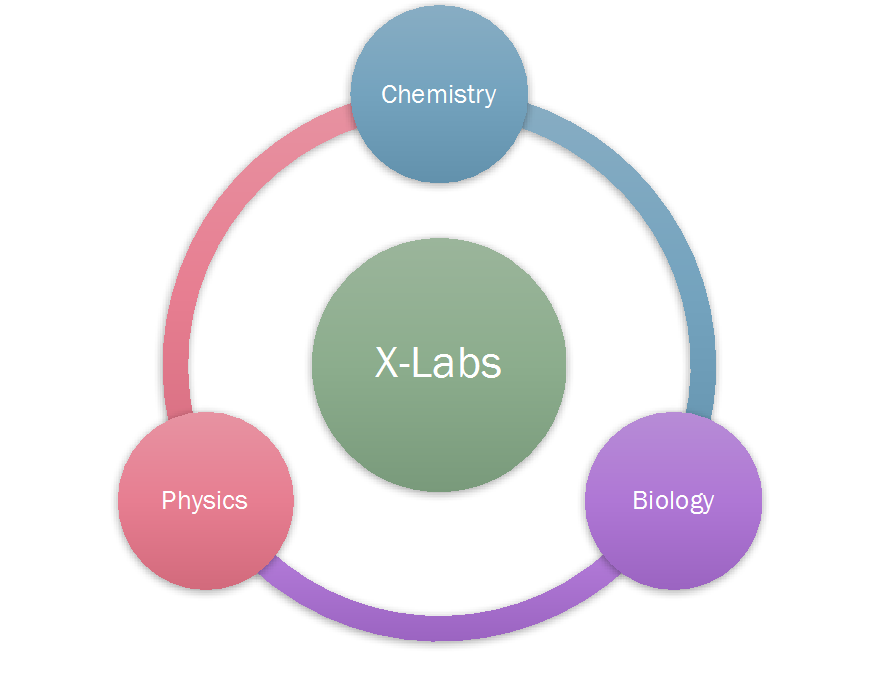
\includegraphics[width=0.5\textwidth,trim = 60 0 70 0, clip]{./logos/xlabsLogo.png}%
      \hfill
\includegraphics[width=0.45\textwidth]{./logos/stemCoreLogoTall.pdf}
    \end{center}
  \end{minipage}

  
  \begin{minipage}{0.25\textwidth}
    \begin{center}\scriptsize
      
\includegraphics[width=0.5\textwidth]{./logos/NSF_4-Color_bitmap_Logo.png}\\
      Award \# 1725655
    \end{center}
  \end{minipage}%
  \begin{minipage}{0.5\textwidth}\scriptsize
    \begin{block}{Project page:}
      \centering \url{https://bit.ly/3k3WoKf}
    \end{block}
  \end{minipage}
\end{frame}

\section{Introduction to ADI}
\begin{frame}{Science Practice Focused Lab curriculum}
  \begin{tabular}{cc}
    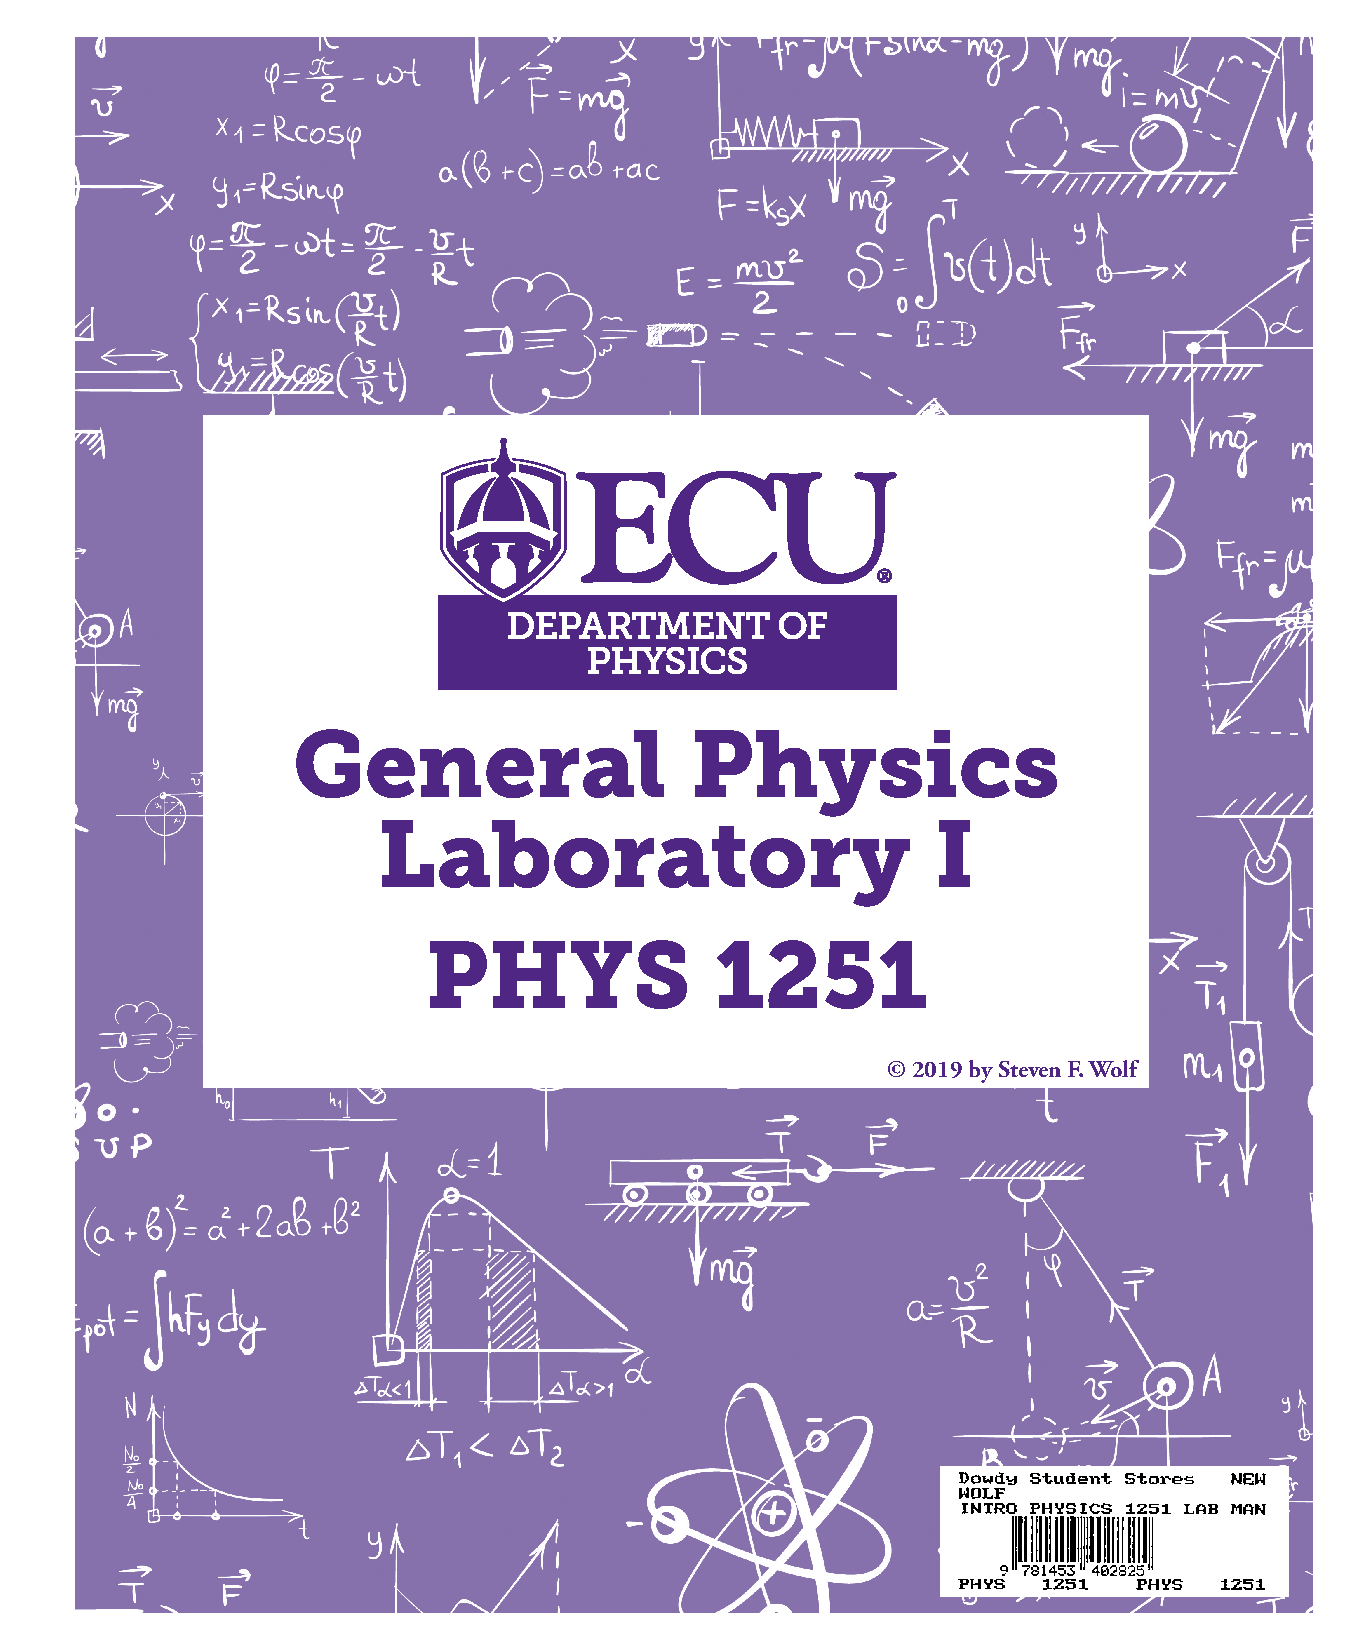
\includegraphics[height=0.6\textheight]{./clipart/p1251cover.pdf}
    &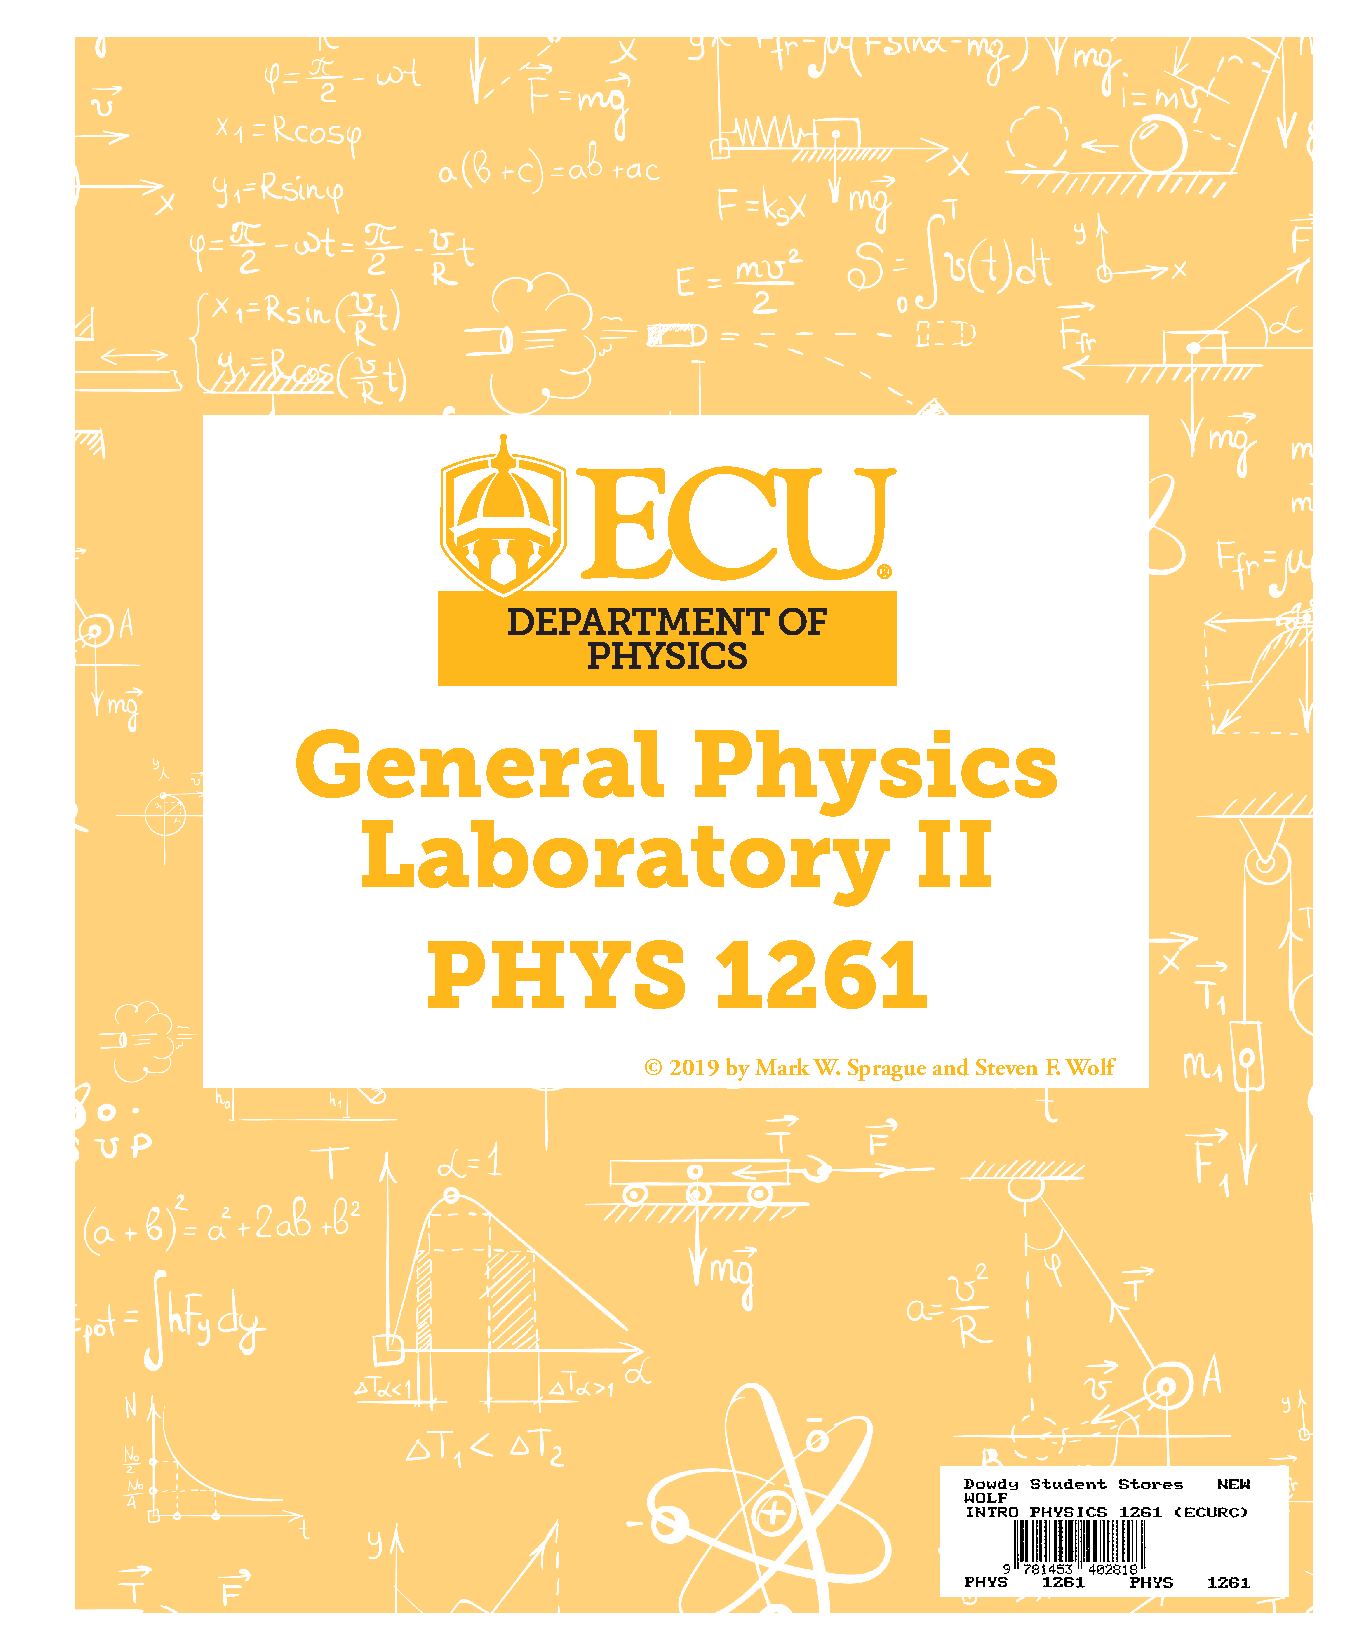
\includegraphics[height=0.6\textheight]{./clipart/p1261cover.pdf} \\
    Piloted Spring 2018 &Piloted Fall 2018 \\
  \end{tabular}
\end{frame}

\begin{frame}{What science practices?}
  \begin{block}{M.J.\ Ford, \textit{Science Education} \textbf{99}, 1041 (2015).}
    \begin{tabular}{lp{4in}} 
      \multicolumn{2}{c}{\textbf{Empirical practices:}} \\
      EP1 &Locate information relevant to a scientific problem.\\
      EP2 &Construct a relevant/appropriate scientific question for a given problem.\\
      EP3 &Design an experiment to test a scientific question.\\
      EP4 &Apply (or know when to apply) appropriate analytical methods to examine a
            scientific problem.\\
      EP5 &Appraise an experimental design to identify elements and limitations and how they
            impact scientific findings/conclusions.\\
      EP6 &Troubleshoot technical issues.\\
      EP7 &Evaluate evidence and critique experimental designs.\\
      EP8 &Interpret basic statistics (e.g., average and SD).\\
    \end{tabular}
  \end{block}
\end{frame}

\begin{frame}{What science practices?}
  \begin{block}{M.J.\ Ford, \textit{Science Education} \textbf{99}, 1041 (2015).}
    \begin{tabular}{lp{4in}} 
      \multicolumn{2}{c}{ \textbf{Representative practices:}} \\
      RP1 &Generate a hypothesis or make a prediction based on a scientific model. \\
      RP2 &Construct an argument based on evidence.\\
      RP3 &Identify additional information needed to support an argument.\\
      RP4 &Provide alternative explanations for results that may have many causes.\\
      RP5 &Integrate and apply knowledge across sub-disciplines.\\
      RP6 &Represent data in a visual form.\\
      RP7 &Interpret visual representations of data.\\
      RP8 &Construct a Data table.\\
      RP9 &Data Analysis.\\
    \end{tabular}
  \end{block}
\end{frame}

{\nologo
  \begin{frame}{Elements of ADI}
    \begin{block}{Week 1: Pre-Lab}
      \begin{minipage}{0.2\textwidth}
        \centering 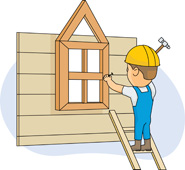
\includegraphics[width=0.9\textwidth]{./clipart/house.jpg}
      \end{minipage}\hfill
      \begin{minipage}{0.75\textwidth}
        \begin{itemize}
          \item Students work in pairs
          \item Learn a new measurement or analysis technique
          \item Traditional lab activity
        \end{itemize}
      \end{minipage}
    \end{block}
    \begin{block}{Week 2: Inquiry Investigation}
      \begin{minipage}{0.75\textwidth}
        \begin{itemize}
          \item Students work in groups of four
          \item Students are given a scientific question to answer
          \item Students design an investigation and carry it out
          \item Investigations must be approved by TA
        \end{itemize}
      \end{minipage}\hfill
      \begin{minipage}{0.2\textwidth}
        \centering 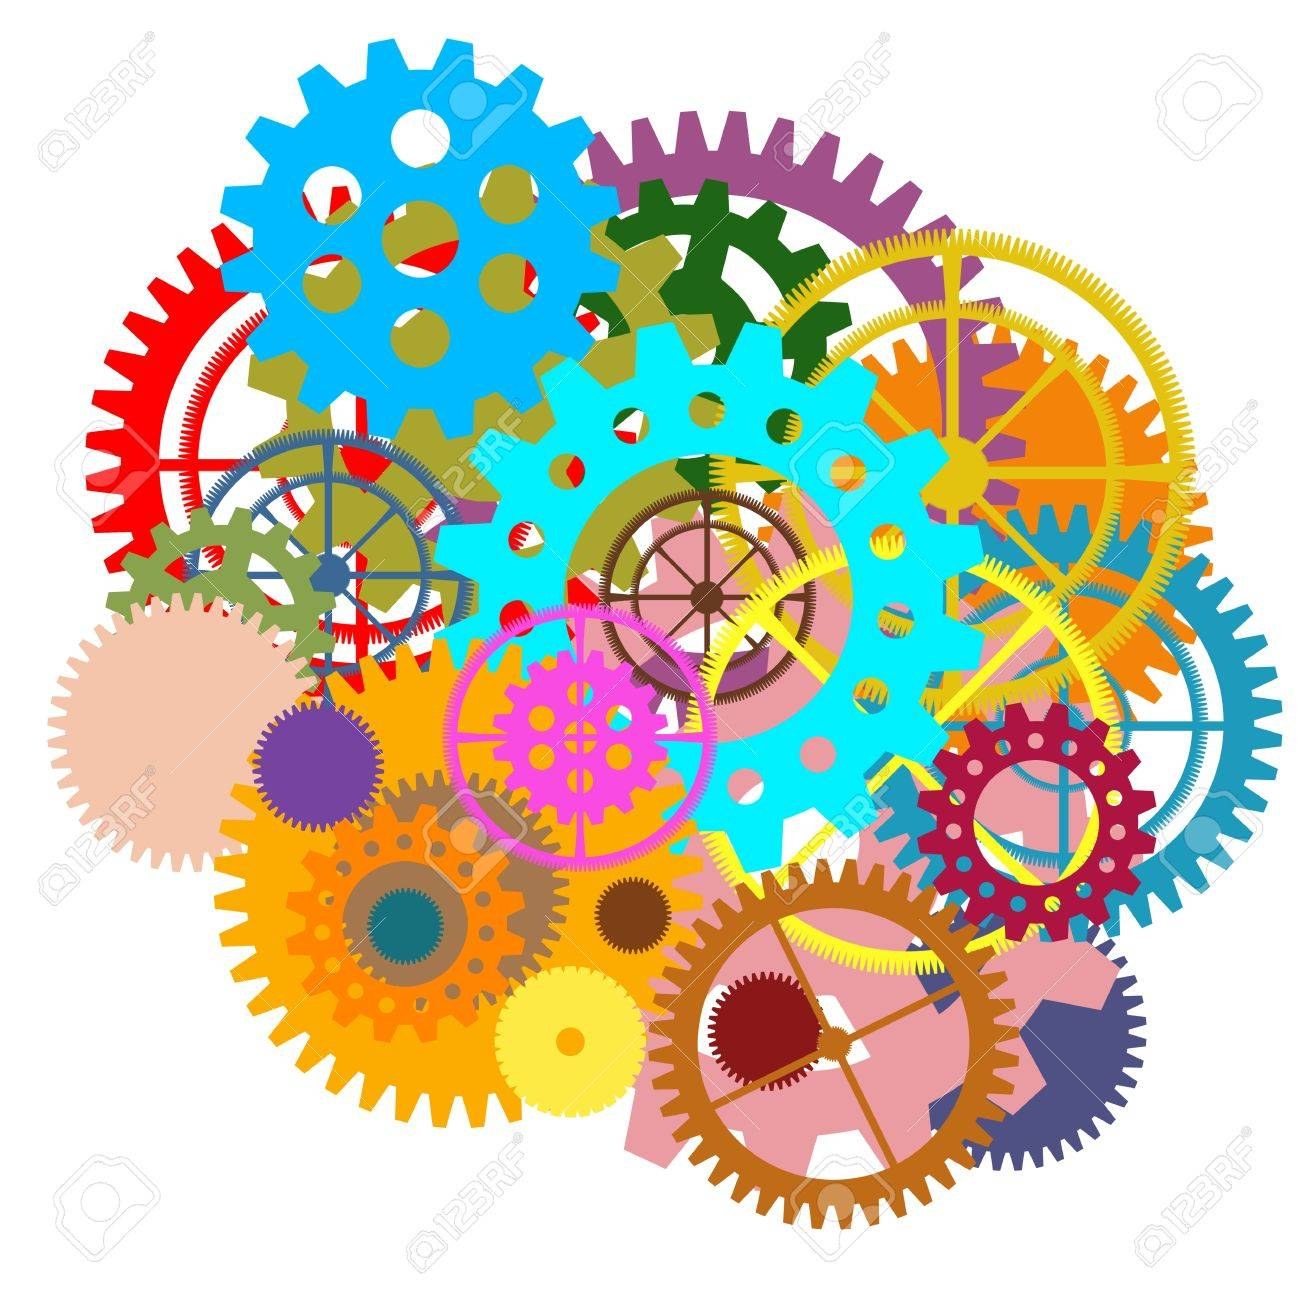
\includegraphics[width=0.9\textwidth]{./clipart/gears.jpg}
      \end{minipage}
    \end{block}
  \end{frame}
}

{\nologo
  \begin{frame}{Elements of ADI}
    \begin{block}{Week 3: Argumentation Session}
      \begin{minipage}{0.2\textwidth}
        \centering 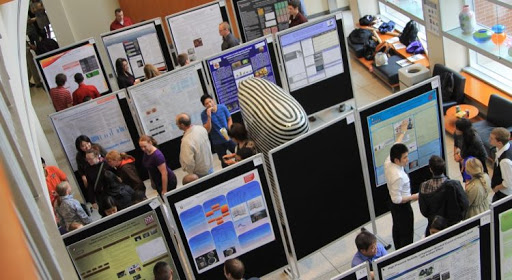
\includegraphics[width=\textwidth]{./clipart/posterSession.jpg}
      \end{minipage}\hfill
      \begin{minipage}{0.75\textwidth}
        \begin{itemize}
          \item Students work in groups of four
          \item Students present the results of their experiment via a ``poster session''
          \item One presenter, three travelers
        \end{itemize}
      \end{minipage}
    \end{block}
    \begin{block}{After Week 3: Peer Review}
      \begin{minipage}{0.75\textwidth}
        \begin{itemize}
          \item Students turn in their first draft after the argumentation session
          \item We use peer review tools embedded in Canvas
          \item Students review 3 papers while watching a peer review calibration video
        \end{itemize}
      \end{minipage}\hfill
      \begin{minipage}{0.2\textwidth}
        \centering 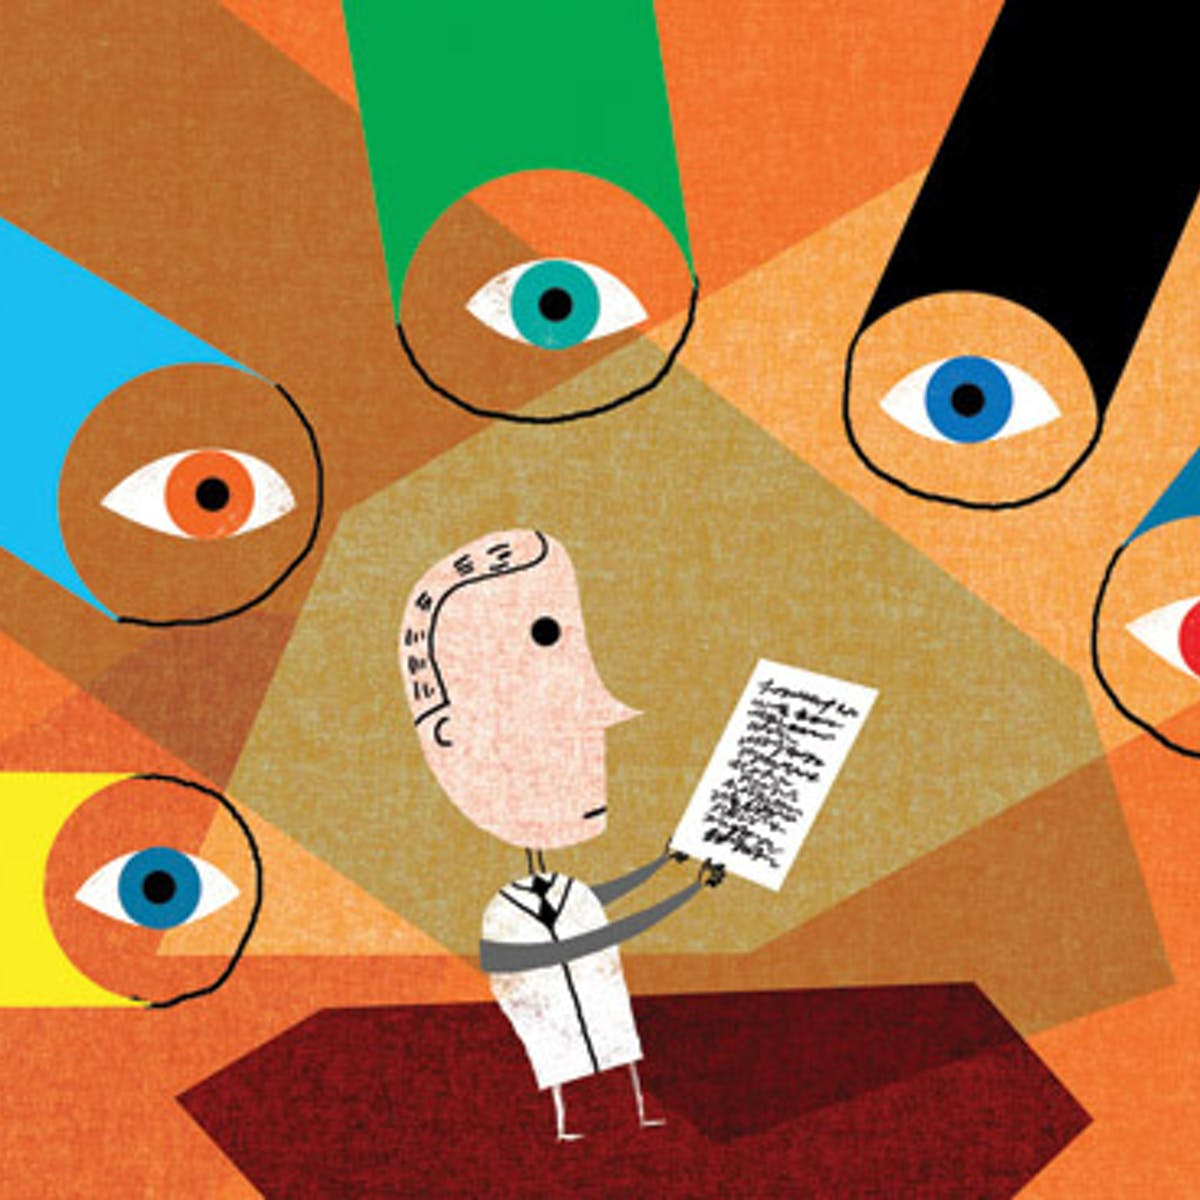
\includegraphics[width=0.9\textwidth]{./clipart/peerReview.jpg}
      \end{minipage}
    \end{block}
  \end{frame}
}

\begin{frame}{Implementation at scale}
  \onslide<1->{
    \begin{block}{Instructional Context}
      Labs serve both Calculus-based and Algebra-based physics lecture courses.
      \begin{description}
        \item[Physics 1] Typically about 400 students in approximately 25 sections managed by
        8-10 TAs.
        \item[Physics 2] Typically about 250 students in approximately 15 sections managed by
        5-6 TAs.
      \end{description}
    \end{block}
  }
  \onslide<2->{
    \begin{block}{Management strategies}
      \begin{itemize}
        \item Course is hosted on our LMS (Canvas) - All sections as one course
        \item Course is set up by lab manager (MWS) - assignments, due dates, syllabus, etc.
        \item All artifacts are turned in online
        \item TAs grade using rubrics\ldots\ calibration is important!
      \end{itemize}
    \end{block}
  }
\end{frame}

\section{Reaction Time Lab Activity}
\begin{frame}{Reaction Time Lab Activity -- Background}
  Plan:
  \begin{itemize}
    \item You will be split into groups of 2 or 3
    \item Your task: Complete the workshop activity on the workshop page
    \item I'm planning 15 minutes for this portion:
    \begin{itemize}
      \item Guidance we give students: 30 data points
      \item We also discuss mean, standard deviation, and standard error
    \end{itemize}
  \end{itemize}

  Link to workshop page:  \url{https://sfwolfphys.github.io/f2020ncsaapt.html}
\end{frame}


\section{Argumentation Session/Reflection}
\begin{frame}{Argumentation Session Instructions -- 15 min}
  Goal:
  \begin{itemize}
    \item Each group will prepare to share out briefly
    \item Want to give you a flavor of how this works in a class
  \end{itemize}
\end{frame}

\section{Online Adaptation}
{\nologo
\begin{frame}{Transition to Online Learning}
  \begin{block}{Spring 2020}
    We had about 2 weeks to plan to finish labs. Keys to success:
    \begin{itemize}
      \item Don't forget about the physics, and your learning goals.
      \item Adapt, don't change.
      \item Get a little lucky.  
    \end{itemize}
  \end{block}
  \begin{block}{Summer 2020 and beyond}
    We still wanted a hands on experience.
    \begin{itemize}
      \item Lab manuals were made available online
      \item Students purchased kits for a reasonable price
    \end{itemize}
    Post pandemic: We have DE students who struggle to take lab courses.
  \end{block}
\end{frame}

\begin{frame}{Online adaptation of ADI Elements}
  \begin{block}{Week 1a and 1b: Pre-Lab}
    \begin{minipage}{0.2\textwidth}
      \centering 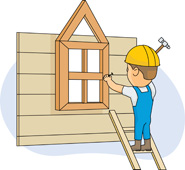
\includegraphics[width=0.9\textwidth]{./clipart/house.jpg}
    \end{minipage}\hfill
    \begin{minipage}{0.75\textwidth}
      \begin{itemize}
        \item TAs hold ``office hours'' at regular class time
        \item Students work asynchronously
      \end{itemize}
    \end{minipage}
  \end{block}
  \begin{block}{Week 2a: Inquiry Investigation}
    \begin{minipage}{0.75\textwidth}
      \begin{itemize}
        \item Students work in groups of four asynchronously
        \item Groups get proposals approved during regular class time
      \end{itemize}
    \end{minipage}\hfill
    \begin{minipage}{0.2\textwidth}
      \centering 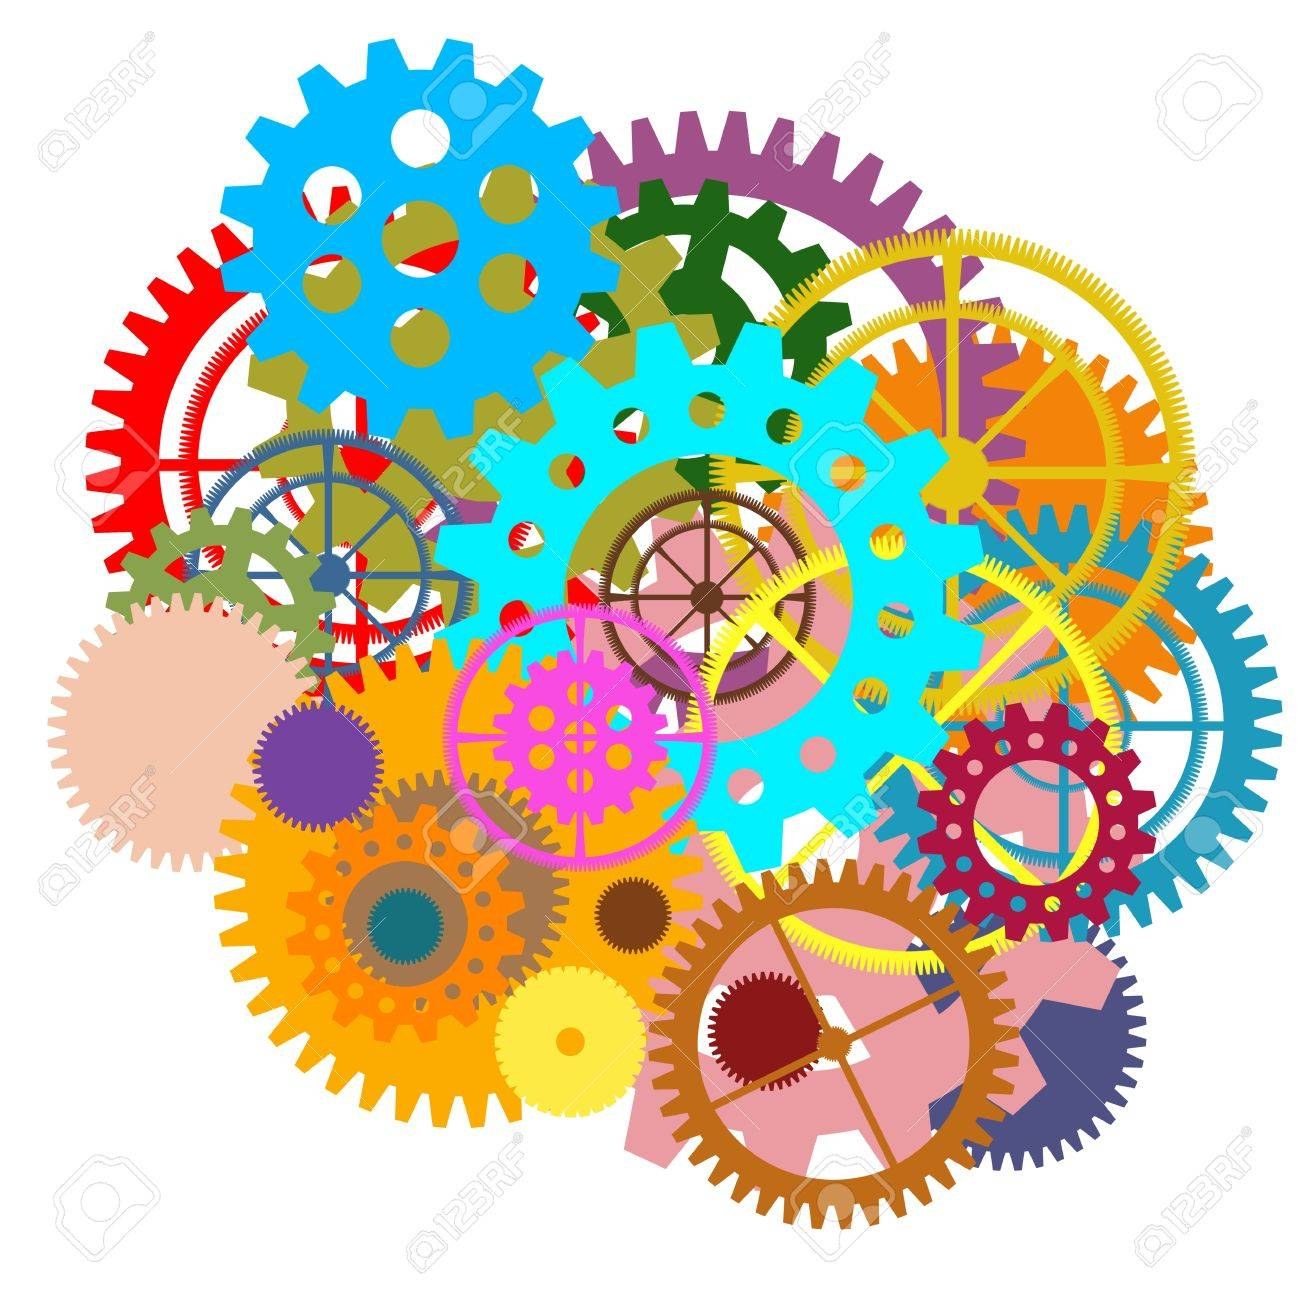
\includegraphics[width=0.9\textwidth]{./clipart/gears.jpg}
    \end{minipage}
  \end{block}
\end{frame}

\begin{frame}{Online adaptation of ADI Elements}
  \begin{block}{Week 2b: Argumentation Session}
    \begin{minipage}{0.2\textwidth}
      \centering 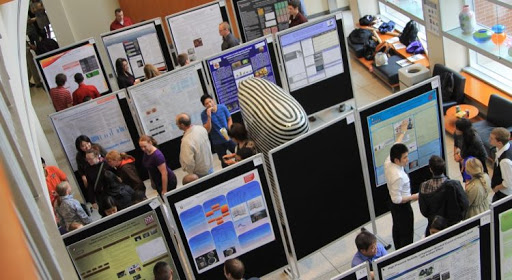
\includegraphics[width=\textwidth]{./clipart/posterSession.jpg}
    \end{minipage}\hfill
    \begin{minipage}{0.75\textwidth}
      \begin{itemize}
        \item Posters are power points rather than whiteboard posters
        \item Argumentation occurs synchronously
      \end{itemize}
    \end{minipage}
  \end{block}
  \begin{block}{After Week 2b: Peer Review}
    \begin{minipage}{0.75\textwidth}
      \begin{itemize}
        \item Remains unchanged
      \end{itemize}
    \end{minipage}\hfill
    \begin{minipage}{0.2\textwidth}
      \centering 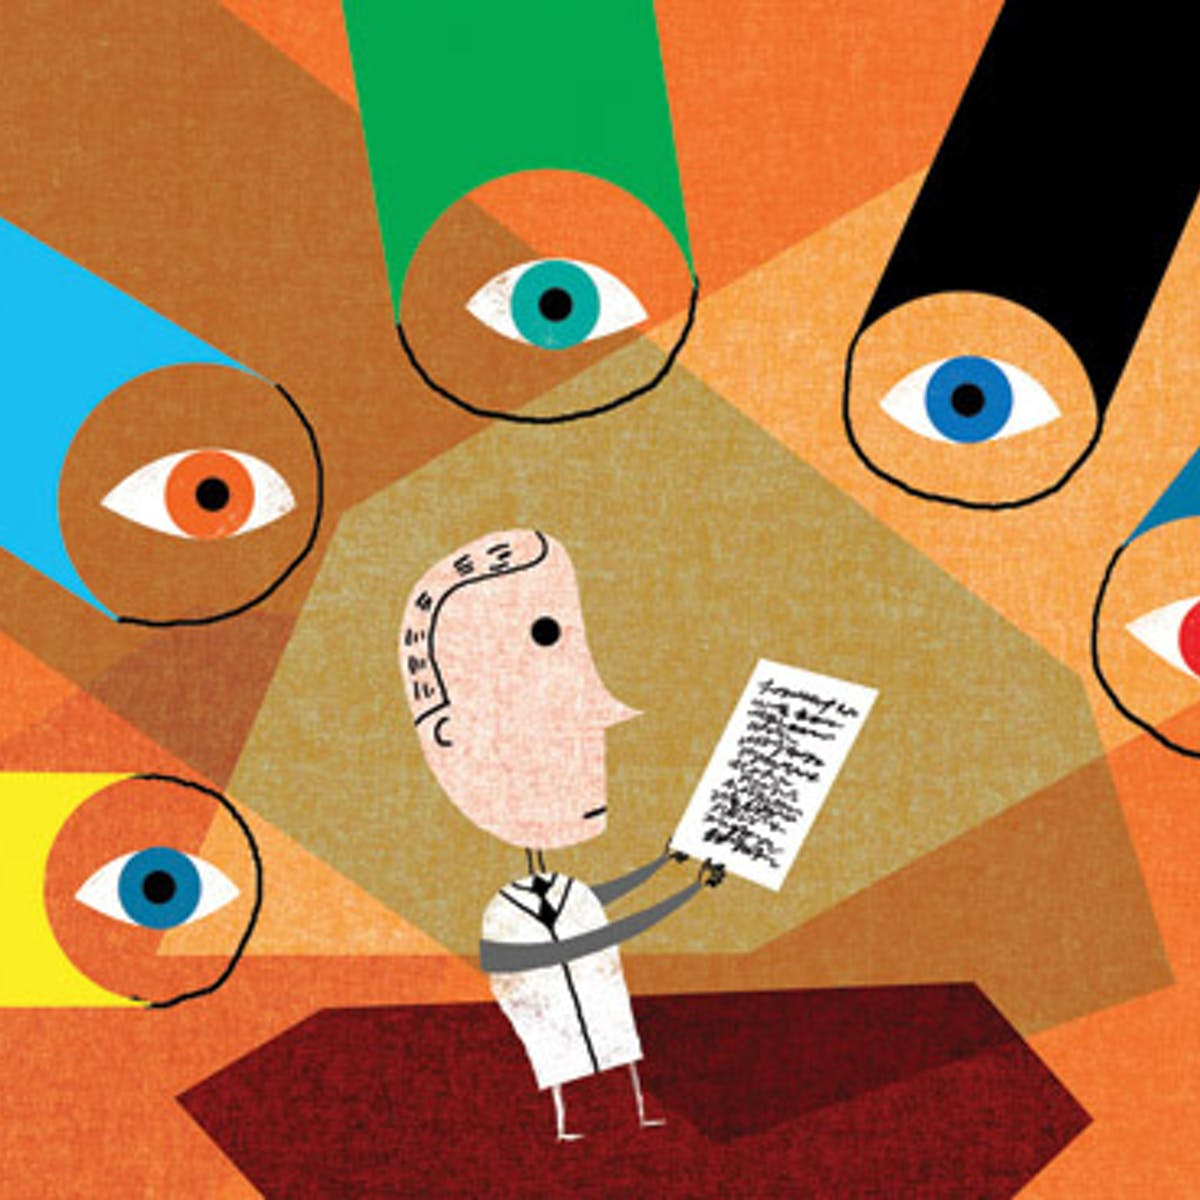
\includegraphics[width=0.9\textwidth]{./clipart/peerReview.jpg}
    \end{minipage}
  \end{block}
\end{frame}
}

\begin{frame}{Physics 1 Online Investigations}
  \begin{center}\scriptsize
    \begin{tabular}{ccp{14em}}
      \hline\hline
      Investigation & Topic & Guiding Question\\
      \hline
      1 & 1-D kinematics & Does a ball rolling on an incline have the same acceleration on the way up as it does on the way down? \\
      2 & 2-D collisions & Is the collision between two marbles elastic? \\
      3 & Periodic motion & What is the nut position for which the physical pendulum small-angle period is minimum, and what is the power-law regression equation for the period of the system? \\
      \hline\hline
    \end{tabular}
  \end{center}
  We have dropped a reaction time investigation due to our shortened semester.
\end{frame}


\begin{frame}{Physics 1 Kit contents}
  \begin{center}
    \begin{tabular}{clc}
      \hline\hline
      Quantity & Item & Investigation(s)\\
      \hline
      1 & Protractor & 1 \\
      2 & \SI{25}{mm} marble & 1, 2 \\
      1 & Tape measure with cm scale & 1, 2, 3\\
      1 & \SI{0.6}{m} threded rod & 3 \\
      1 & Eye nut & 3 \\
      3 & Nuts & 3 \\
      1 & Door hook & 3 \\
      1 & \SI{1}{m} string & 3 \\
      1 & \SI{16}{mm} marble & 2 \\
      \hline\hline
    \end{tabular}
  \end{center}
\end{frame}

\begin{frame}
  {Physics 2 Online Investigations}
  \begin{center}
    \begin{tabular}{ccp{12em}}
      \hline\hline
      Investigation & Topic & Guiding Question\\
      \hline
      1 & Current and resistance & Does a light bulb behave like a resistor? \\
      2 & Time varying circuits & Do two of the lab kit capacitors have the same capacitance? \\
      3 & Diffraction of light & Are hairs from different people the same diameter? \\
      \hline\hline
    \end{tabular}
  \end{center}
\end{frame}

\begin{frame}{Physics 2 kit contents}
  \begin{center}\scriptsize
    \begin{tabular}{clc}
      \hline\hline
      Quantity & Item & Investigation(s)\\
      \hline
      1 & \SI{100}{\ohm} resistor & 1 \\
      1 & \SI{330}{\ohm} resistor & 1 \\
      1 & \SI{100}{\ohm} potentiometer & 1 \\
      1 & E10 light bulb holder & 1 \\
      1 & \SI{5}{V} E10 incandescent light bulb & 1 \\
      1 & Breadboard & 1, 2, 3 \\
      1 & Breadboard power supply & 1, 2, 3 \\
      1 & USB power supply cable & 1, 2, 3 \\
      1 & Jumper wire set & 1, 2 \\
      2 & Multimeters & 1, 2 \\
      1 & Mini screwdriver for multimeters & 1, 2 \\
      5 & \SI{500}{mA} fuses for multimeters & 1, 2 \\
      4 & Alligator clip leads & 1, 2 \\
      1 & \SI{1}{\mega\ohm} resistor & 2 \\
      2 & \SI{100}{\micro\farad} capacitor & 2 \\
      1 & \SI{5}{V}, \SI{650}{nm} laser module & 3 \\
      1 & Tape measure with cm scale & 3 \\            
      \hline\hline
    \end{tabular}
  \end{center}

\end{frame}

\begin{frame}{}
  \vfill \centerline{\Huge Thank You!}  \vfill \centerline{\Large Any Questions?}
  \vfill
  \begin{textblock*}{0.5\textwidth}(5mm,82mm) \textblockcolor{} {\scriptsize
      \url{wolfs15@ecu.edu} }
  \end{textblock*}
\end{frame}



% {\nologo
% % \begin{frame}[allowframebreaks]{References}
%   \begin{frame}{References}

%     {\scriptsize \bibliographystyle{apsrev} \bibliography{biblio} }
%   \end{frame}
% }

\end{document}
